\documentclass[compress]{beamer}
\usepackage{ifthen,verbatim}

\newcommand{\isnote}{}
\xdefinecolor{lightyellow}{rgb}{1.,1.,0.25}
\xdefinecolor{darkblue}{rgb}{0.1,0.1,0.7}
\xdefinecolor{darkgreen}{rgb}{0.,0.4,0.}

%% Uncomment this to get annotations
%% \def\notes{\addtocounter{page}{-1}
%%            \renewcommand{\isnote}{*}
%% 	   \beamertemplateshadingbackground{lightyellow}{white}
%%            \begin{frame}
%%            \frametitle{Notes for the previous page (page \insertpagenumber)}
%%            \itemize}
%% \def\endnotes{\enditemize
%% 	      \end{frame}
%%               \beamertemplateshadingbackground{white}{white}
%%               \renewcommand{\isnote}{}}

%% Uncomment this to not get annotations
\def\notes{\comment}
\def\endnotes{\endcomment}

\setbeamertemplate{navigation symbols}{}
\setbeamertemplate{headline}{\mbox{ } \hfill
\begin{minipage}{5.5 cm}
\vspace{-0.75 cm} \small
\end{minipage} \hfill
\begin{minipage}{4.5 cm}
\vspace{-0.75 cm} \small
\begin{flushright}
\ifthenelse{\equal{\insertpagenumber}{1}}{}{Jim Pivarski \hspace{0.2 cm} \insertpagenumber\isnote/\pageref{numpages}}
\end{flushright}
\end{minipage}\mbox{\hspace{0.2 cm}}\includegraphics[height=1 cm]{../cmslogo} \hspace{0.1 cm} \includegraphics[height=1 cm]{../tamulogo} \hspace{0.01 cm} \vspace{-1.05 cm}}

\begin{document}
\begin{frame}
\vfill
\begin{center}
\textcolor{darkblue}{\Large Effect of misalignment on tracks for MPOG Note}

\vspace{0.2 cm}
\textcolor{darkblue}{\Large and CRUZET endcap alignment results}

\vfill
\begin{columns}
\column{0.3\linewidth}
\begin{center}
{\Large
\textcolor{darkblue}{Jim Pivarski}}

\vspace{0.2 cm}
Alexei Safonov
\end{center}

%% \column{0.3\linewidth}
%% \begin{center}
%% \large
%% K\'aroly Banicz
%% \end{center}
\end{columns}

\begin{columns}
\column{0.3\linewidth}
\begin{center}
\scriptsize
{\it Texas A\&M University}
\end{center}
%% \column{0.3\linewidth}
%% \begin{center}
%% \scriptsize
%% {\it US-CMS}
%% \end{center}
\end{columns}

\vfill
18 August, 2008

\end{center}
\end{frame}

%% \begin{notes}
%% \item This is the annotated version of my talk.
%% \item If you want the version that I am presenting, download the one
%% labeled ``slides'' on Indico (or just ignore these yellow pages).
%% \item The annotated version is provided for extra detail and a written
%% record of comments that I intend to make orally.
%% \item Yellow notes refer to the content on the {\it previous} page.
%% \item All other slides are identical for the two versions.
%% \end{notes}

\begin{frame}
\frametitle{Two topics}
\begin{itemize}\setlength{\itemsep}{1 cm}
\item Quantified effect of residual misalignment on tracks for MPOG Note, using CSA08 results

\item Aligned CSC disks in CRUZETs 1\&2

\vspace{0.1 cm}
\begin{itemize}
\item Status of CRUZET-3 and prompt AlCaReco for CRUZET-4
\end{itemize}
\end{itemize}
%% \hspace{-0.83 cm} \textcolor{darkblue}{\Large Outline2}
\end{frame}

\begin{frame}
\frametitle{Misalignment Scenarios}
\begin{itemize}\setlength{\itemsep}{0.5 cm}
\item \textcolor{darkblue}{Estimated hardware-only alignment:} Gaussian-distributed
  misalignments with sigmas on the order of those expected from
  hardware systems only (LAS in tracker, MHAS in muon system), also
  known as STARTUP scenario

\item \textcolor{darkblue}{Estimated 10~pb$^{-1}$ scenario:} Gaussian-distributed
  misalignments with sigmas expected from inclusion of track-based
  alignment; used in some Monte Carlo samples

\item \textcolor{darkblue}{Result of 10~pb$^{-1}$ exercise:} residual misalignments after
  CSA08 exercises (tracker and muon system), also known as S156

\item \textcolor{darkblue}{Perfect alignment,} also known as ideal
\end{itemize}
\end{frame}

\begin{frame}
\frametitle{Curvature resolution}
\small
\vspace{0.2 cm}
(Fractional uncertainty in $1/p_T$ equals fractional uncertainty in $p_T$)
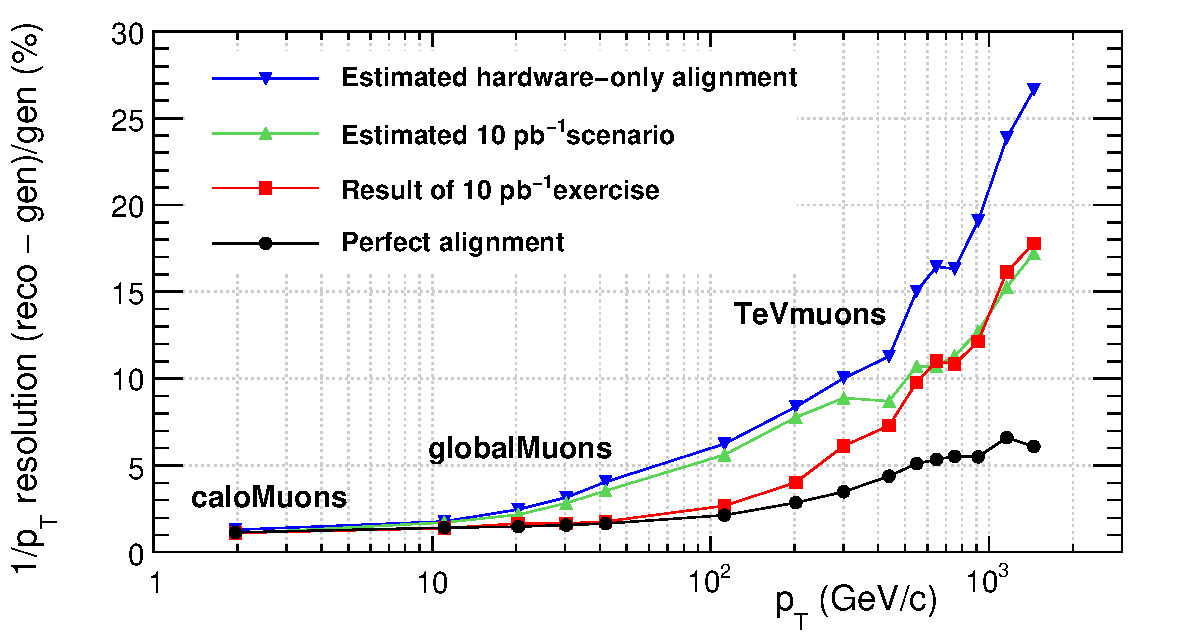
\includegraphics[width=\linewidth]{curvature_resolution.pdf}

\vspace{-0.3 cm}
\begin{itemize}
\item caloMuons below 5~GeV, globalMuons below 50~GeV, TeVmu/firstHit above
\item \textcolor{red}{CSA08 tracker results} much better than \textcolor{darkgreen}{10~pb$^{-1}$ estimate} because MinBias were more useful than expected
\end{itemize}
\end{frame}

\begin{frame}
\frametitle{Split up by $\eta$}

\begin{columns}
\column{0.33\linewidth}
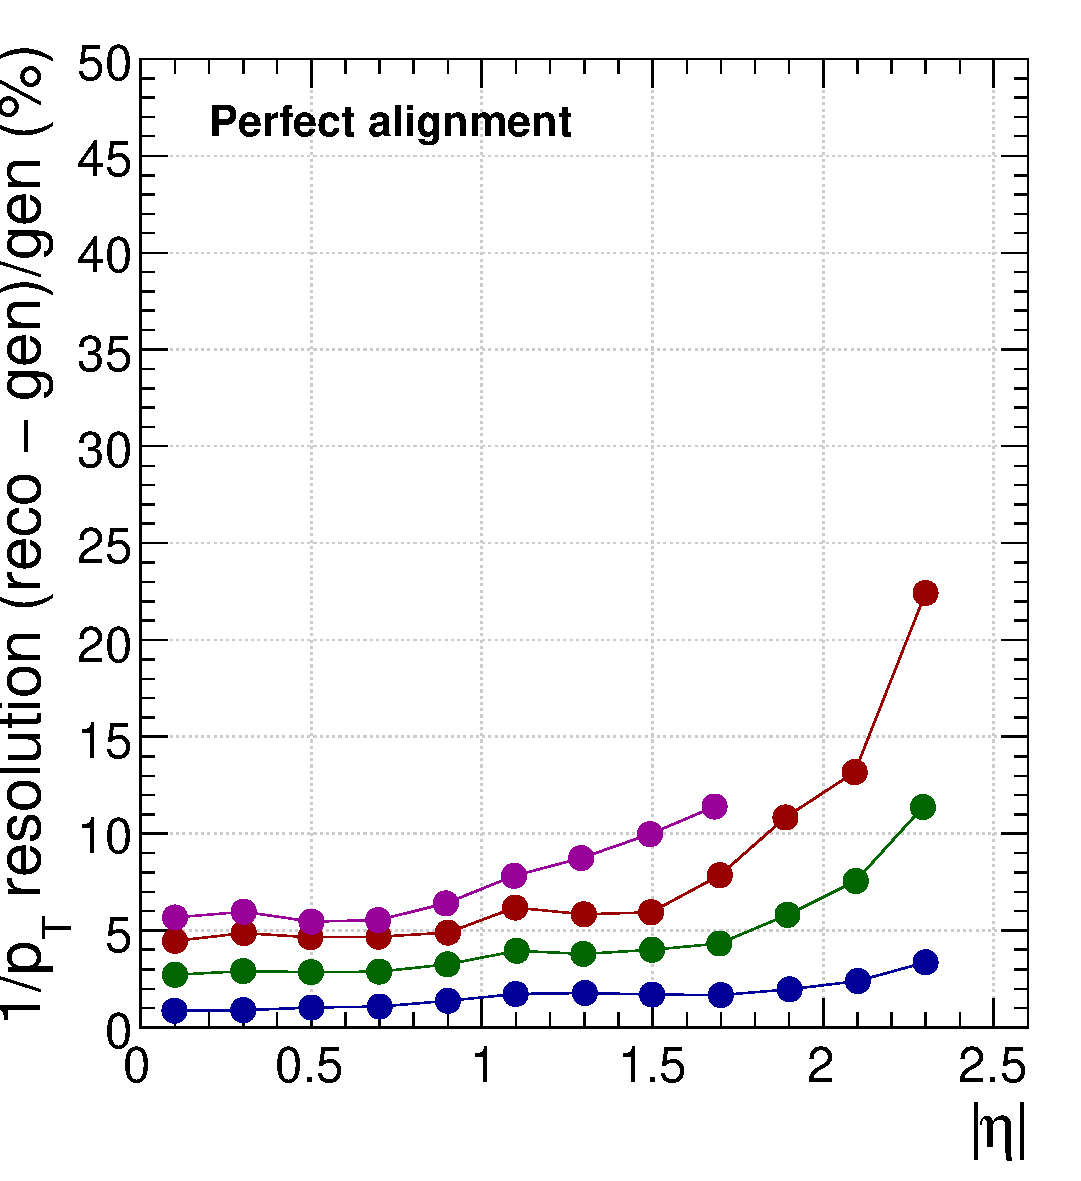
\includegraphics[width=\linewidth]{curvature_byeta_ideal.pdf}
\column{0.33\linewidth}
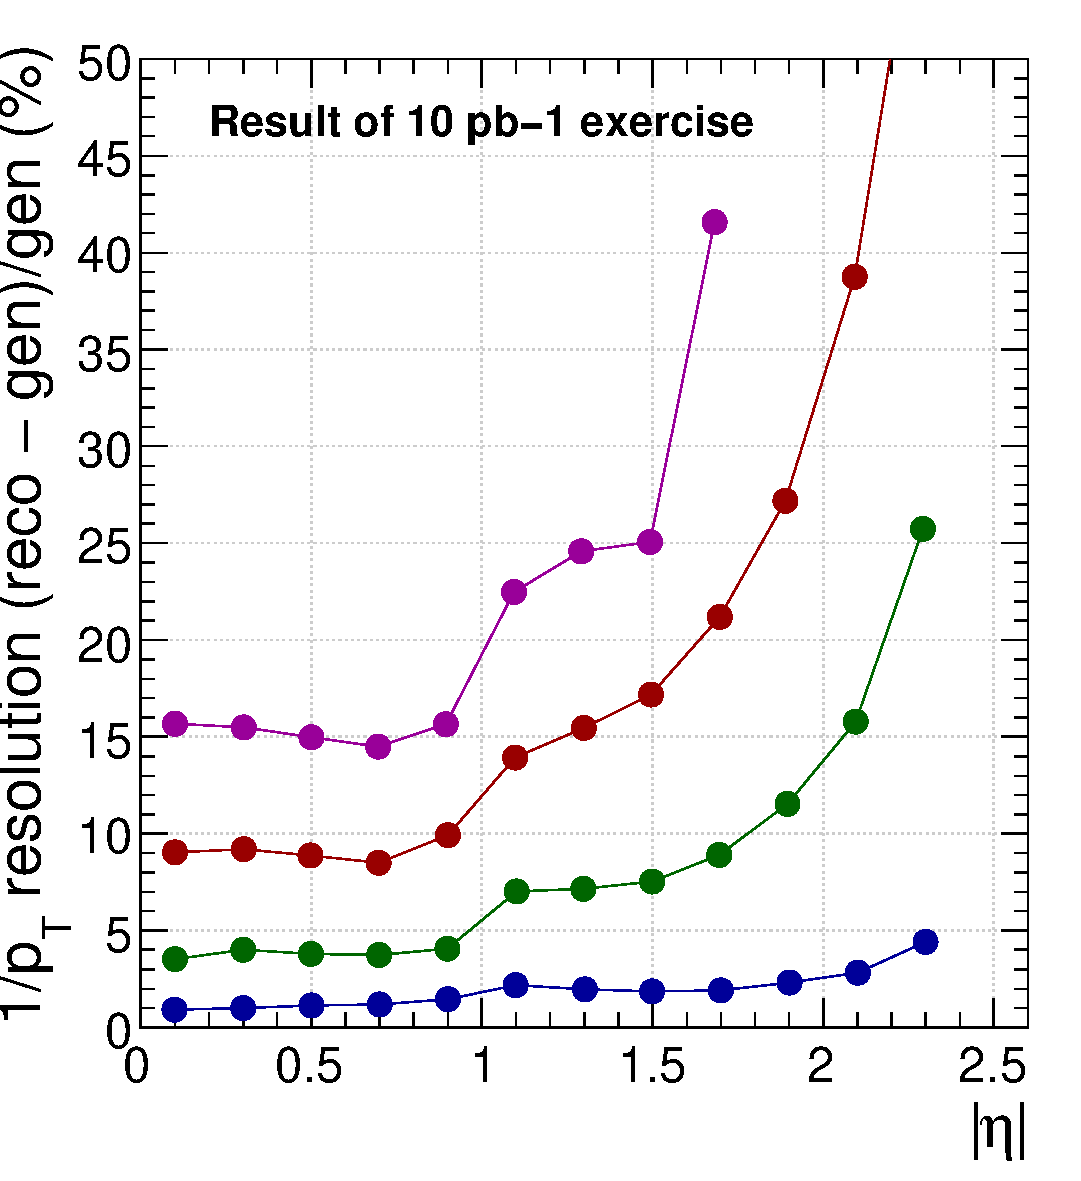
\includegraphics[width=\linewidth]{curvature_byeta_csa.pdf}
\column{0.33\linewidth}
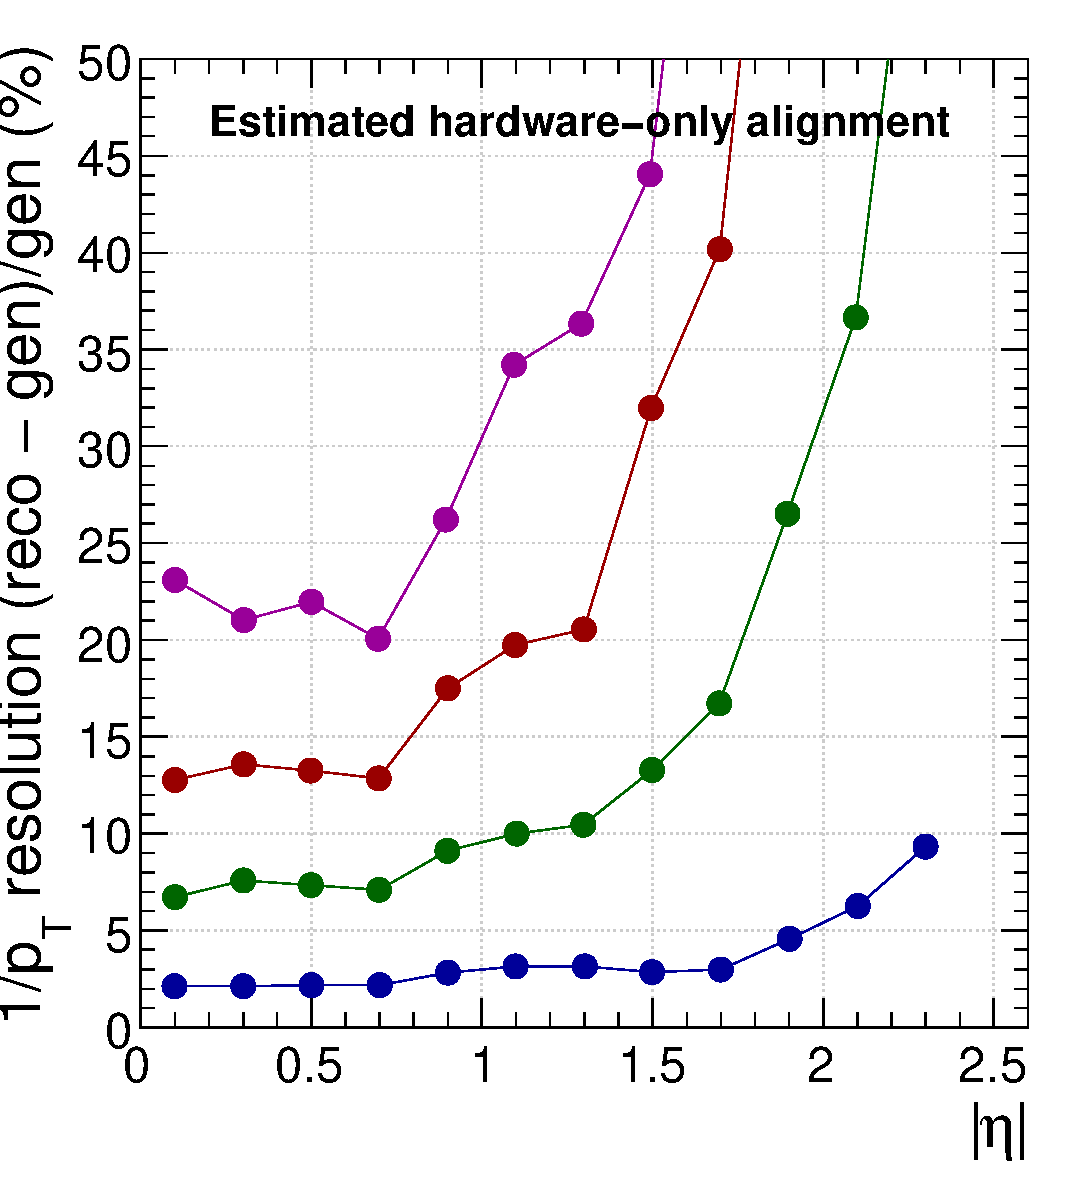
\includegraphics[width=\linewidth]{curvature_byeta_zero.pdf}
\end{columns}

{\hspace{-0.5 cm} \small Bottom-to-top: \textcolor{blue}{$<$ 50~GeV (blue),} \textcolor{darkgreen}{$<$ 500 (green),} \textcolor{red}{$<$ 1000 (red),} \textcolor{violet}{\mbox{above (purple) \hspace{-2 cm}}}}

\vspace{0.3 cm}
\begin{columns}
\column{0.28\linewidth}
Muon alignment:

\vspace{0.2 cm}
\scriptsize Alignment accuracy a little better at high $\eta$, but radial lever arm for measuring $p_T$ is several times smaller

\column{0.75\linewidth}
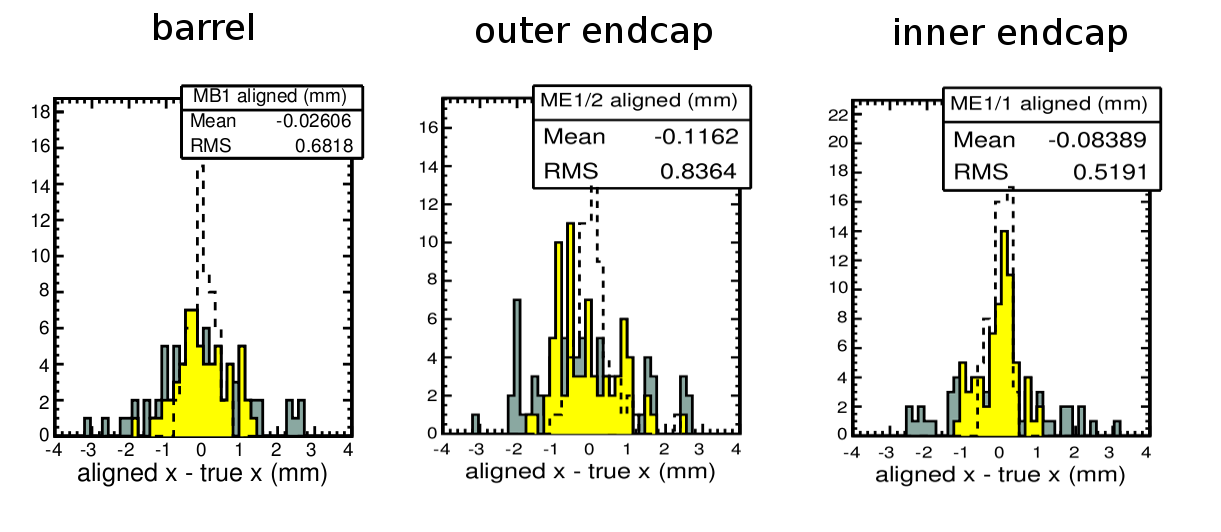
\includegraphics[width=\linewidth]{muonhip_barrel-endcap.png}
\end{columns}

\scriptsize Grey: hardware-only, \fbox{yellow: 10~pb$^{-1}$ track-based,} dashed: same \mbox{with perfect tracker\hspace{-1 cm}}
\end{frame}

\begin{frame}
\frametitle{Mass resolution}

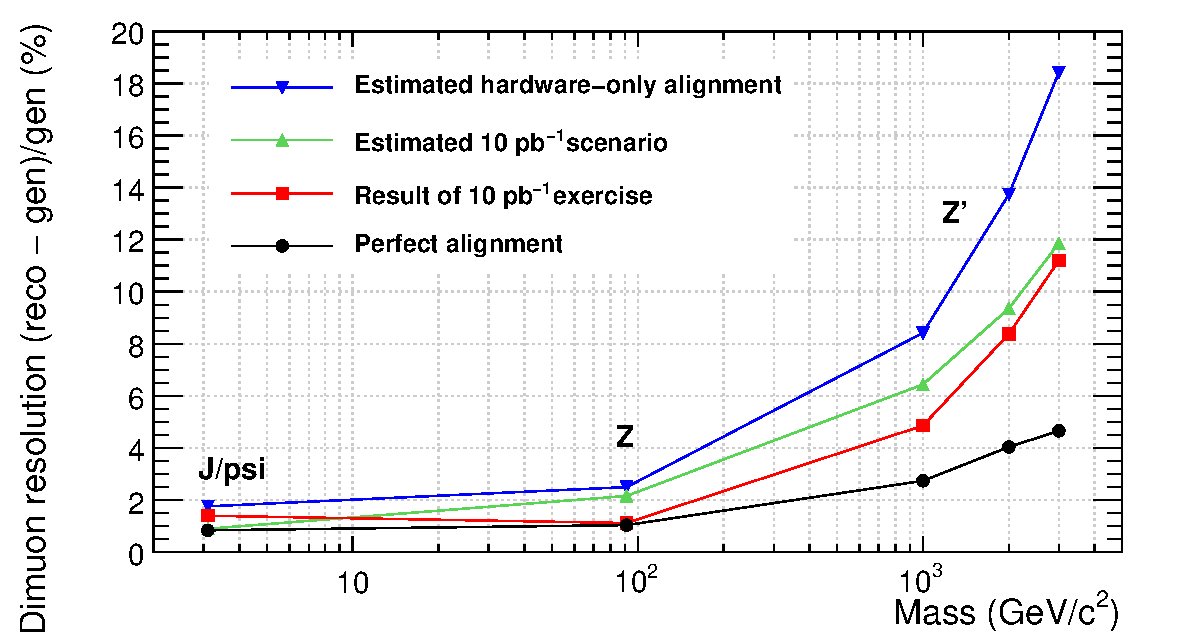
\includegraphics[width=\linewidth]{mass_resolution.pdf}

\vspace{0.5 cm}
\begin{itemize}\setlength{\itemsep}{0.2 cm}
\item $\Delta p_T$ is smaller at low masses

\item $\Delta \phi$, $\Delta \eta$ are smaller at high masses
\end{itemize}
\end{frame}

\begin{frame}
\frametitle{CRUZET Alignments}
\small

\vspace{0.2 cm}
Endcap disk alignment for CRUZETs 1\&2 (no tracker)

\vspace{0.4 cm}
\hspace{-0.83 cm} \textcolor{darkblue}{\Large Method:}

\begin{itemize}
\item Muon barrel is the (aligned) reference
\item Fit tracks in one tracking volume (barrel or a CSC disk), align
  a more-distant disk using those tracks
\end{itemize}

\begin{center}
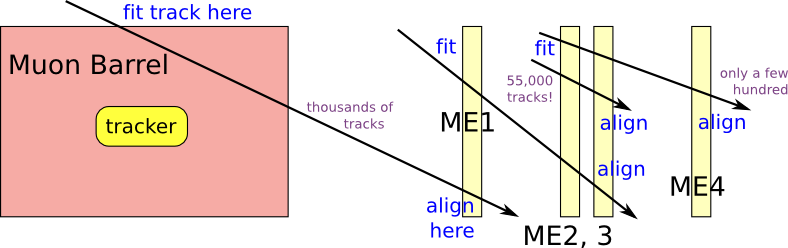
\includegraphics[width=0.8\linewidth]{fit_here_align_there.png}
\end{center}

\vspace{-0.4 cm}
\begin{itemize}
\item Allows for internal cross-checks: compare direct MB $\to$ ME2

against MB $\to$ ME1 $+$ ME1 $\to$ ME2 (etc.)

\item Uses standard alignment framework in a non-standard way
\end{itemize}
\end{frame}

\begin{frame}
\frametitle{Results for CRUZETs 1\&2}
\small

\begin{columns}
\column{0.64\linewidth}
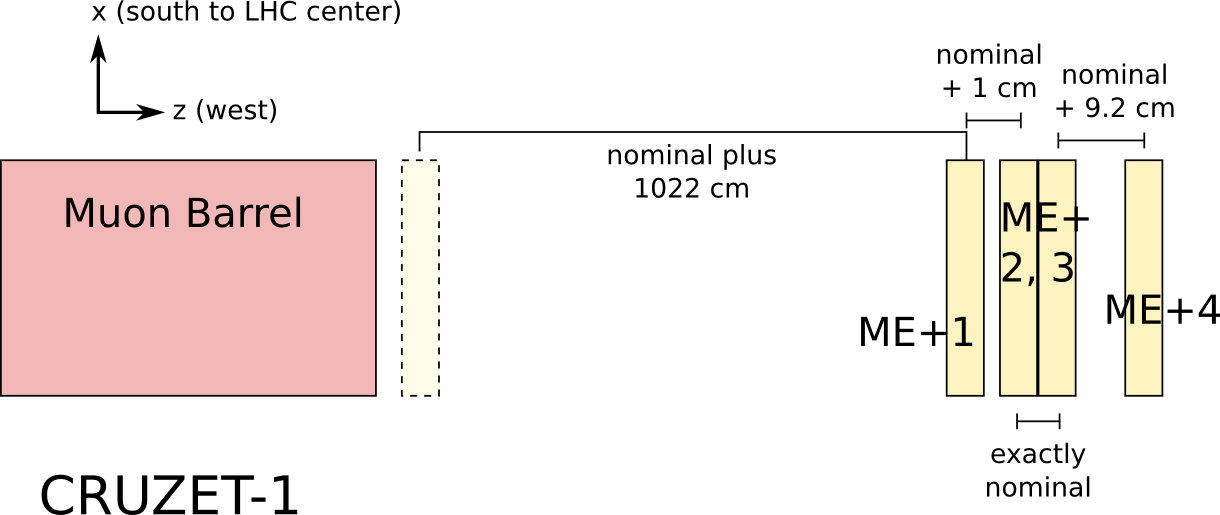
\includegraphics[height=3 cm]{cruzet1_results.png}

\vspace{0.5 cm}
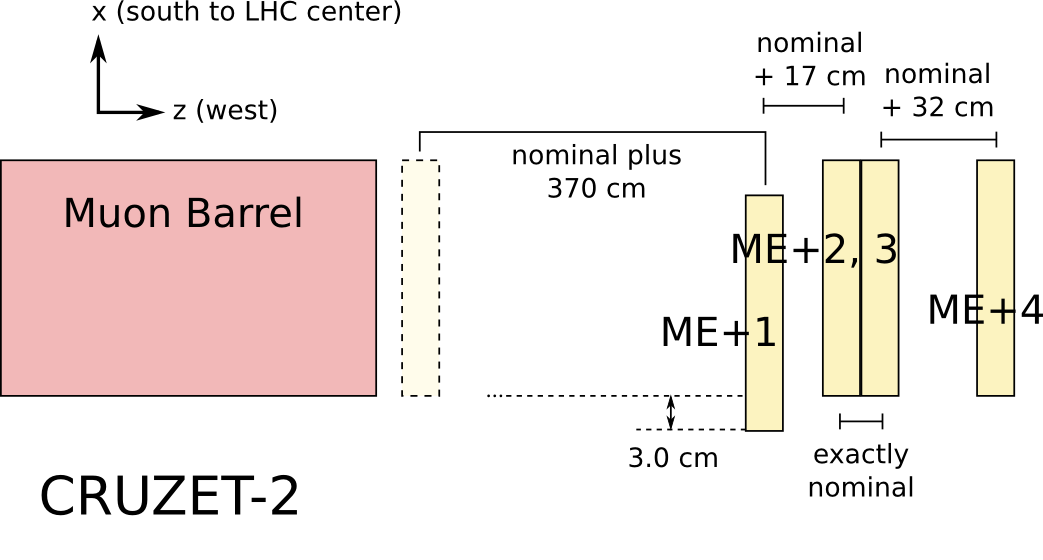
\includegraphics[height=3.3 cm]{cruzet2_results.png}

\column{0.4\linewidth}

\vspace{0.35 cm}
Tags for CSCAlignmentRcds in database (with IOVs):

\vspace{0.2 cm}
{\tt \tiny CRUZET1-CSCStation-xyz-2mmRadialFix\_v1

CRUZET2-CSCStation-xyzphiz-2mmRadialFix\_v2}

\vspace{0.4 cm}
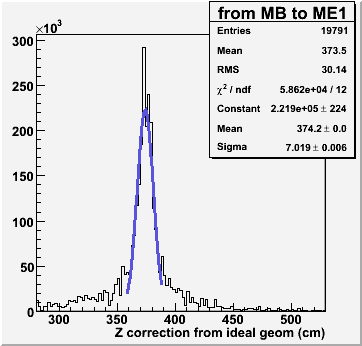
\includegraphics[width=\linewidth]{hist_0and1.png}

\end{columns}

\vspace{0.4 cm}
Requires approx.\ position of endcap; displacements between \mbox{disks are new\hspace{-1 cm}}

\vspace{0.2 cm}
Details (soon): \textcolor{blue}{\tt \scriptsize \underline{\href{https://twiki.cern.ch/twiki/bin/view/CMS/MuonAlignment}{https://twiki.cern.ch/twiki/bin/view/CMS/MuonAlignment}}}

\end{frame}

\begin{frame}
\frametitle{Consistency checks}
\small

\begin{center}
\begin{tabular}{c | c c c c}
\scriptsize Comparison & \scriptsize $x$ (mm) & \scriptsize $y$ (mm) & \scriptsize $z$ (mm) & \scriptsize $\phi_z$ (mrad) \\\hline
\scriptsize (MB$\to$2) $-$ (MB$\to$1$\to$2) & \scriptsize -12.8 & \scriptsize 6.4 & \scriptsize 39.9 & \scriptsize -4.75 \\
\scriptsize (MB$\to$3) $-$ (MB$\to$2$\to$3) & \scriptsize -3.4 & \scriptsize -8.7 & \scriptsize -15.3 & \scriptsize -1.06 \\
\scriptsize (MB$\to$4) $-$ (MB$\to$3$\to$4) & \scriptsize 0.4 & \scriptsize 6.0 & \scriptsize 10.3 & \scriptsize 2.8 \\\hline
\end{tabular}
\end{center}

\vspace{0.1 cm}
\[ \sqrt{\frac{1}{N-1} \sum (x_i - \bar{x})^2} = \left\{\begin{array}{l} \mbox{7.8~mm for $x$ and $y$} \\ \mbox{28~mm for $z$} \\ \mbox{3.8~mrad for $\phi_z$} \end{array}\right. \]

\vspace{0.1 cm}
Some values verified with physical measurements (tape measure)

\vspace{0.3 cm}
\hspace{-0.83 cm} \textcolor{darkblue}{\Large Follow-ups:}

\begin{itemize}\setlength{\itemsep}{0.1 cm}
\item Apply same procedure to CRUZET-3 after re-reco (status?)
\item Validate CRUZET-4 prompt AlCaReco
\item Use tracker in CRUZETs 3\&4 as a reference
\item Depending on statistics and quality of tracker tracks, apply
  chamber-by-chamber alignment procedure
\end{itemize}
\end{frame}

\begin{frame}
\frametitle{Conclusions}
\begin{itemize}\setlength{\itemsep}{0.75 cm}
\item MPOG Note estimates of momentum resolution based on from CSA08 alignment exercises

\item Aligned CRUZETs 1\&2 disks, same procedure ready for 3\&4

\item Tracker-to-muon and chamber-by-chamber alignments will also be possible in 3\&4

\item CRUZET-4 will also test prompt AlCaReco (StandAloneMuons and GlobalMuons)
\end{itemize}
\label{numpages}
\end{frame}

\end{document}
